\documentclass[11pt]{article}

\usepackage[T1]{fontenc}
\usepackage{lmodern}
\usepackage{microtype}
\usepackage[margin=1in]{geometry}
\usepackage{amsmath,amssymb,amsthm,mathtools}
\usepackage{booktabs,tabularx,array}
\usepackage{enumitem}
\usepackage[dvipsnames]{xcolor}
\usepackage{tikz}
\usetikzlibrary{arrows.meta,positioning,calc}
\usepackage{natbib}
\usepackage[colorlinks=true,linkcolor=MidnightBlue,citecolor=BrickRed,
  urlcolor=MidnightBlue]{hyperref}
\usepackage[nameinlink,noabbrev]{cleveref}
\usepackage{fancyhdr}

\definecolor{NCSBlue}{HTML}{173B57}
\definecolor{NCSGold}{HTML}{B57A17}
\definecolor{NCSGray}{HTML}{F1F4F6}
\definecolor{NCSRed}{HTML}{8D2E2E}

\newtheorem{theorem}{Theorem}[section]
\newtheorem{proposition}[theorem]{Proposition}
\newtheorem{lemma}[theorem]{Lemma}
\newtheorem{corollary}[theorem]{Corollary}
\theoremstyle{definition}
\newtheorem{definition}[theorem]{Definition}
\newtheorem{example}[theorem]{Example}
\theoremstyle{remark}
\newtheorem{remark}[theorem]{Remark}

\newcommand{\Path}{\operatorname{Path}}
\newcommand{\Dom}{\operatorname{Dom}}
\newcommand{\Lip}{\operatorname{Lip}}
\newcommand{\dist}{\operatorname{dist}}
\newcommand{\Exact}{\operatorname{Exact}}
\newcommand{\ord}{\operatorname{ord}}
\newcommand{\id}{\mathrm{id}}
\newcommand{\R}{\mathbb{R}}
\newcommand{\N}{\mathbb{N}}
\newcommand{\cK}{\mathcal{C}_K}
\newcommand{\vdef}{\mathsf{V}}
\newcommand{\afail}{\mathsf{A}}
\newcommand{\cfail}{\mathsf{C}}

\setlist{itemsep=0.25em,topsep=0.4em}
\setlength{\parskip}{0.25em}
\setlength{\parindent}{1.2em}
\setlength{\emergencystretch}{3em}

\pagestyle{fancy}
\fancyhf{}
\fancyhead[L]{\footnotesize Noncommutative comparative statics}
\fancyhead[R]{\footnotesize Research-program paper}
\fancyfoot[C]{\thepage}
\renewcommand{\headrulewidth}{0.3pt}

\title{\vspace{-1.5em}
{\color{NCSBlue}\bfseries Noncommutative Comparative Statics}\\[0.35em]
\large A defect calculus for order-sensitive adjustment protocols}
\author{Independent Research Program}
\date{27 July 2026}

\begin{document}
\maketitle

\begin{abstract}
Many constrained systems do not simply jump to a uniquely selected optimum
when their external conditions change. They carry their current state
forward, make a locally economical repair, and retain the residue of earlier
repairs. Two externally compatible interventions can therefore produce
different outcomes, or different feasibility, when applied in different
orders. We propose \emph{noncommutative comparative statics} (NCS) as a
mathematical research program centered on this phenomenon.

The basic model is a presented category of external interventions together
with a response functor from its free path category to metric spaces and
partial Lipschitz maps. A relation cell declares two intervention paths
externally equivalent; the response need not satisfy that relation. We
separate directional route-asymmetric failure, common failure, and finite
value discrepancy. Signed-distance predicate robustness supplies a precise
baseline: a finite route difference can become one-sided infeasibility under
a later partial response only near the continuation domain's feasibility
boundary. We give its one-step two-sided boundary-exposure form and use it in
a three-intervention example. We also define an amplitude-calibrated reporting
order, which distinguishes the quadratic small cells of smooth connection
curvature from linear active-set effects and order-zero jumps.

The paper imports, rather than relabels as new, quantitative rewriting,
Hyers--Ulam rectification, predicate robustness, discrete connections, ordered
projection, hybrid-system, and comparative-statics results. An
affine-contractive relation operator gives a computable baseline
rectification problem, including noninvertible maps. Exact
configuration-repair and online-allocation examples show how the same
definitions report finite order debt and hard feasibility asymmetry. The
proposed contribution is an explicitly delimited shared modeling framework,
falsification protocol, and research agenda---not a novelty claim for
noncommutativity, curvature, margins, confluence, or sequential recourse.
\end{abstract}

\noindent\textbf{Keywords.}
comparative statics; partial maps; adjustment cost; path dependence;
quantitative rewriting; active sets; algorithmic recourse; Ulam stability.

\vspace{0.8em}
\begin{center}
\begin{minipage}{0.92\textwidth}
\colorbox{NCSGray}{%
\parbox{0.96\textwidth}{\small
\textbf{Status and priority boundary.}
This is a proposal for a field and a first foundations paper, not a claim that
the field is already established. A mapped literature search found no source
packaging the full response/failure/scaling framework below, but every major
mathematical ingredient has close antecedents. No theorem in this paper by
itself establishes a separate field. The proposal is limited to the combined
intervention/response schema, directional reporting convention,
cross-sector falsification protocol, and research agenda.}}
\end{minipage}
\end{center}

\section{The missing question}

Classical comparative statics asks how an equilibrium or optimizer changes
with an external parameter. This is exactly the right question when the model
specifies a unique state \(x^\ast(b)\) for every parameter \(b\). It is not the
right question for a stateful repair protocol.

Consider a system with a current feasible state. A requirement changes. The
system minimizes disruption from \emph{where it currently is}, rather than
re-solving from a timeless reference. A second requirement then arrives and
the system repairs again. Even if the final set of requirements is independent
of their order, the accumulated state need not be.

This motif recurs in technical problem solving:

\begin{itemize}
  \item a configuration manager preserves earlier edits while satisfying a
  new constraint;
  \item an allocation system admits arrivals without moving incumbents;
  \item a biological or engineered redundant system redistributes internal
  load as its environment changes;
  \item an active-set optimizer crosses different constraint faces in
  different orders;
  \item a person follows sequential algorithmic-recourse recommendations.
\end{itemize}

The pattern is especially salient in requests of the form ``change this one
thing while keeping everything else consistent.'' It appears across learned
problem-solving corpora and across fields, but each field gives it a different
mathematical home. The proposal here is to make the \emph{composition of
response protocols} the primary object.\footnote{This is a hypothesis drawn
from recurring problem structures, not an inspection of individual neural
network weights.}

The under-formalized claim is therefore organizational and empirical, not
that partial maps or noncommuting operators were unknown. Models commonly
specify either the external endpoint, the internal dynamics, or the failure
rule. NCS asks them to specify together (i) which intervention paths are
externally equivalent, (ii) how current state is carried along each path, and
(iii) which directional failure and value discrepancies are measured when
the response does not respect that equivalence.

\begin{table}[t]
\centering
\caption{Classical and noncommutative comparative statics ask different
questions.}
\label{tab:questions}
\begin{tabularx}{\textwidth}{>{\bfseries}p{0.24\textwidth}XX}
\toprule
 & Classical comparative statics & NCS \\
\midrule
State semantics & selected equilibrium \(x^\ast(b)\) &
current state plus an adjustment protocol \\
Primary comparison & two external endpoints &
two externally equivalent paths \\
Failure & often excluded by regularity &
an observable distinct from value error \\
Path independence & built into a state function &
a property to test or rectify \\
Local diagnostic & derivative of \(x^\ast\) &
relation-cell response signature \\
\bottomrule
\end{tabularx}
\end{table}

\subsection{Reset and carry}

The first conceptual distinction is simple and non-negotiable.

\begin{description}
\item[Reset response.] Recompute a distinguished state from a fixed reference
for every new external condition. A unique reset state is a section and is
path-independent by construction.
\item[Carry response.] Repair from the current state. Earlier accommodations
remain unless a later requirement forces them to change.
\end{description}

Confusing these semantics creates a false theorem: a unique static argmin
cannot acquire holonomy merely because its derivative is written
geometrically. NCS treats reset and carry as different response functors on
the same feasible fibers.

\section{Position among established fields}

The proposed field sits at an interface. This section records the collisions
that determine what may and may not be claimed.

\paragraph{Comparative statics and recourse.}
Monotone comparative statics is a mature theory
\citep{milgrom1994}; adjustment costs have been incorporated explicitly
\citep{dekel2025}; and ``recourse'' has long-standing meanings in stochastic
programming \citep{dantzig1955}. Sequential and ordered algorithmic recourse
is also established \citep{rasouli2024,verma2022}. NCS does not claim that
order-sensitive adjustment is undiscovered. It seeks a common defect language
for the response maps those models generate.

\paragraph{Rewriting and concurrency.}
A pair of competing response paths is a quantitative diamond. Adjacent swaps
of independent actions are the basis of trace theory
\citep{mazurkiewicz1988}, directed concurrency
\citep{kahl2016,earnshaw2026}, and quantitative rewriting
\citep{gavazzo2023}. Metric-enriched categories already express
approximately commuting diagrams \citep{kubis2013}. Accordingly, the
triangle-inequality accumulation bound in \cref{sec:filling} is a baseline,
not a headline result.

\paragraph{Connections and holonomy.}
Horizontal lift, curvature, and holonomy are classical
\citep{ehresmann1952,ambrose1953,oneill1966}. In redundant robotics,
minimum-norm feasible velocity is explicitly the pseudoinverse horizontal lift
\citep{altafini2004,shamir1988}. Discrete edge transport and plaquette
curvature are likewise established
\citep{leok2005,fernandez2022,wilson1974}. The smooth sector of NCS is a
reduction to this theory.

\paragraph{Moving constraints and hybrid seams.}
Sweeping processes model motion constrained by a moving set
\citep{moreau1977}; rate-independent systems model incremental dissipation and
hysteresis \citep{mielke2004}; and projection algorithms already study
ordered noninvertible operators \citep{bauschke1996}. Exit-path categories and
hybrid systems model noninvertible cross-stratum transport and saltation
products \citep{treumann2009,woolf2009,burden2016,kong2024}. Scattering
diagrams organize path-ordered wall products and joint consistency
\citep{gross2018}. NCS adds no canonical seam map to a stratification; the
response protocol must supply it.

\paragraph{Predicate robustness and partial maps.}
Distance to a predicate boundary as a truth-preserving robustness radius is
established in metric temporal logic and hybrid systems
\citep{fainekos2009}. Boundary-band risk is also standard in robust
classification \citep{zhang2019trades}, while convergence theories compare
partial maps through both their domains and values \citep{beer2014}.
Accordingly, the guard lemma in \cref{sec:seam} and its one-step
boundary-exposure estimate are imported baselines. Their role is to connect
those quantities to competing adjustment paths, not to rename them as new
mathematics.

\paragraph{Rectification and Ulam stability.}
The question ``does almost satisfying the relations imply proximity to an
exact representation?'' is Ulam stability
\citep{burger2010,gowers2015,voiculescu1983,becker2023,arzhantseva2015}.
For a Hilbert operator, the optimal residual-to-kernel error constant is the
norm of its Moore--Penrose inverse \citep{huang2012}. We use this theorem as a
computational baseline for an affine response sector; we do not present it as
a new rectification theorem.

\section{Presented interventions and response functors}

\subsection{External intervention syntax}

\begin{definition}[weighted intervention presentation]
An intervention presentation
\[
K=(K_0,K_1,K_2,\{p_\sigma\Rightarrow q_\sigma\},w_1,w_2)
\]
consists of a finite directed graph, a finite family of pairs of nonempty
parallel paths, and positive edge and cell weights. The cell
\(p_\sigma\Rightarrow q_\sigma\) declares that the two paths have the same
net external meaning.
\end{definition}

Let \(\Path(K)\) be the free category on the graph and set
\[
\cK=\Path(K)/\langle p_\sigma=q_\sigma:\sigma\in K_2\rangle.
\]
The quotient is the external intervention category. The presentation matters:
it records which changes are elementary, which exchanges are operationally
meaningful, and how evidence is weighted. It is not merely a redundant
description of \(\cK\).

\begin{figure}[t]
\centering
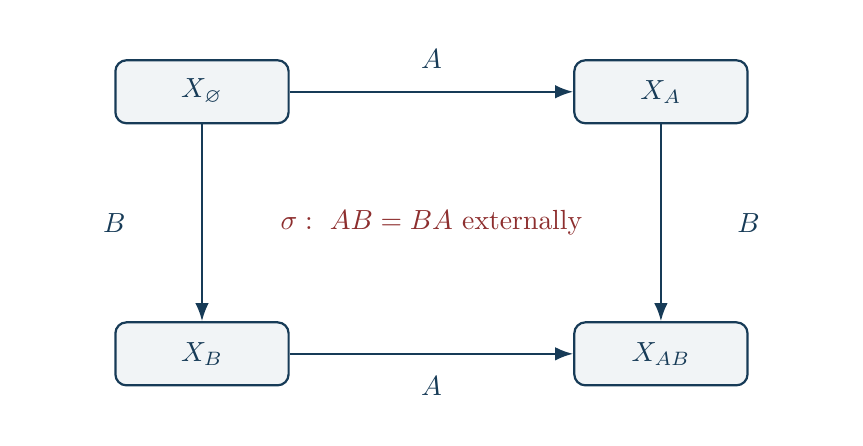
\begin{tikzpicture}[
  node distance=2.5cm and 3.6cm,
  every node/.style={draw=NCSBlue,rounded corners,fill=NCSGray,
    minimum width=2.2cm,minimum height=0.8cm,align=center},
  every path/.style={-{Latex[length=2.3mm]},thick,NCSBlue}
]
\node (o) {\(X_{\varnothing}\)};
\node (a) [right=of o] {\(X_A\)};
\node (b) [below=of o] {\(X_B\)};
\node (ab) [right=of b] {\(X_{AB}\)};
\draw (o) -- node[above,draw=none,fill=none] {\(A\)} (a);
\draw (o) -- node[left,draw=none,fill=none] {\(B\)} (b);
\draw (a) -- node[right,draw=none,fill=none] {\(B\)} (ab);
\draw (b) -- node[below,draw=none,fill=none] {\(A\)} (ab);
\node[draw=none,fill=none,text=NCSRed] at ($(o)!0.5!(ab)$)
  {\(\sigma:\ AB=BA\) externally};
\end{tikzpicture}
\caption{A relation cell equates two external intervention orders. The
response maps on the four edges need not make the state square commute.}
\label{fig:square}
\end{figure}

\subsection{Partial Lipschitz response}

\begin{definition}[partial Lipschitz map]
A partial Lipschitz map \(T:X\rightharpoonup Y\) is a subset
\(\Dom T\subseteq X\) and a map \(T:\Dom T\to Y\) for which some finite
\(L\) satisfies
\[
d_Y(Tx,Tx')\le Ld_X(x,x')
\]
whenever \(d_X(x,x')<+\infty\). Its modulus \(\Lip(T)\) is the infimum
of such \(L\). Composition has domain
\[
\Dom(S\circ T)=\{x\in\Dom T:T(x)\in\Dom S\}.
\]
These arrows form the category \(\mathbf{pMetPar}_{\mathrm{Lip}}\).
\end{definition}

\begin{definition}[response assignment]
A deterministic response assignment is a functor
\[
R:\Path(K)\longrightarrow\mathbf{pMetPar}_{\mathrm{Lip}}.
\]
It is \emph{exact} relative to \(K\) if it factors through \(\cK\).
\end{definition}

The pair \((K,R)\) is the basic \emph{NCS model}. A statistical study also
declares input measures and value scales; a scaling study additionally
declares physical intervention amplitudes. These choices are part of the
model, not canonical decorations.

The Lipschitz target is intentionally wider than nonexpansive response.
A unique optimizer need not depend nonexpansively on its reference state.
Smooth horizontal transports between fibers with changing metrics need not be
nonexpansive either. The model must prove or record the relevant local
Lipschitz modulus.

\subsection{Morphisms and gauge}

An \emph{unweighted semantic morphism}
\((F,\eta):(K,R)\to(K',R')\) contains a functor
\(F:\Path(K)\to\Path(K')\) satisfying
\[
F(p_\sigma)\sim_{K'}F(q_\sigma)
\]
for every relation and a natural transformation
\(\eta:R\Rightarrow R'F\) with total finite-Lipschitz components in the
partial-map category. Mapping an edge to a path permits operational
refinement. This notion forgets \(w_1,w_2\). A quantitative morphism would
also need chosen target derivations and bounds on edge-path and cell-weight
distortion; we leave its canonical formulation open.

A gauge equivalence fixes the intervention presentation and uses fiberwise
bijective isometries. It preserves route domains and value distances.
Uniformly bi-Lipschitz fiber changes give two-sided distortion bounds.
Presentation equivalence, quotient-category equivalence, and response gauge
equivalence are different notions.

\section{A failure-aware order signature}

Let \(p,q:a\to b\) be parallel intervention paths and let
\(D_p=\Dom R_p\), \(D_q=\Dom R_q\).

\begin{definition}[domain/value signature]
The deterministic order signature is
\begin{align*}
\afail^+_{p,q}&=D_p\setminus D_q,
&
\afail^-_{p,q}&=D_q\setminus D_p,\\
\cfail_{p,q}&=X_a\setminus(D_p\cup D_q),
&
\vdef_{p,q}(x)&=d_b(R_px,R_qx),
\quad x\in D_p\cap D_q.
\end{align*}
\end{definition}

The four entries distinguish:

\begin{enumerate}
  \item only the first order succeeds;
  \item only the second order succeeds;
  \item both orders fail;
  \item both succeed but disagree in value.
\end{enumerate}

A single extended distance that assigns \(+\infty\) to one-sided failure and
zero to common failure is convenient algebraically but scientifically
incomplete. In particular, universal failure is path-independent and useless.

For a probability measure \(\mu\) on \(X_a\) and a truncation scale \(M>0\),
define the directional empirical signature
\begin{align}
A_\mu^+(p,q)&=\mu(D_p\setminus D_q),\label{eq:asymplus}\\
A_\mu^-(p,q)&=\mu(D_q\setminus D_p),\label{eq:asymminus}\\
C_\mu(p,q)&=\mu(\cfail_{p,q}),\label{eq:common}\\
V_{\mu,M}(p,q)&=
\int_{D_p\cap D_q}
\min\left\{1,\frac{d_b(R_px,R_qx)}{M}\right\}\,d\mu(x).
\label{eq:value}
\end{align}
This produces the directly estimable order signature
\((A_\mu^+,A_\mu^-,C_\mu,V_{\mu,M})\). Write
\[
A_\mu^{\leftrightarrow}=A_\mu^++A_\mu^-
=\mu(D_p\triangle D_q)
\]
when only total asymmetry is needed. Retaining the two directions is
essential: their sum cannot say which order fails.

This convention is useful rather than mathematically exotic. Totalize a
partial map by an undefined state \(\bot\), put
\(d_M^\bot(y,y')=\min\{1,d(y,y')/M\}\), and set
\(d_M^\bot(y,\bot)=1\). Then
\[
\int d_M^\bot(\widehat p,\widehat q)\,d\mu
=A_\mu^{\leftrightarrow}+V_{\mu,M},
\]
while \(C_\mu\) is common-\(\bot\) mass. Thus the signature is a
scientifically interpretable decomposition of standard objects, not a claim
of a new metric on partial maps.

\begin{proposition}[exact descent]
\label{prop:descent}
The response \(R\) factors through \(\cK\) if and only if every relation cell
has equal route domains and zero value defect on that domain.
\end{proposition}

\begin{proof}
The condition is equality of the corresponding partial maps. The universal
property of the presented category gives the factorization.
\end{proof}

Common failure is compatible with exact descent, which is why it must be
retained as a separate performance observable.

\section{Baseline filling calculus}
\label{sec:filling}

Suppose \(P_0=p,\ldots,P_N=q\) is a relation-cell swap derivation at \(x\) and
every intermediate route is defined at \(x\). At step \(i\), write the two
routes as a common prefix \(a_i\), alternative cell sides \(u_i,v_i\), and a
common suffix \(b_i\). Choose a positive finite Lipschitz bound
\(L_{b_i}>0\) for each suffix response. Using chosen positive bounds avoids
the indeterminate product \(0\cdot+\infty\) allowed by extended metrics.

\begin{proposition}[admissible derivation bound]
\label{prop:filling}
\[
d(R_px,R_qx)\le
\sum_{i=0}^{N-1}
L_{b_i}\,
d(R_{u_i}R_{a_i}x,R_{v_i}R_{a_i}x).
\]
\end{proposition}

\begin{proof}
Use the triangle inequality across successive route outcomes and propagate
each local comparison through its common suffix.
\end{proof}

The response filling cost is the infimum of the right-hand side over
\emph{admissible} derivations and valid positive suffix bounds. It is
\(+\infty\) if none exists. Ordinary combinatorial filling area is safe only
for total responses or after a domain-robustness theorem. This distinction is
essential: a small local value difference can straddle the domain of a later
partial map and become one-sided failure.

\section{Imported guard robustness and boundary exposure}
\label{sec:seam}

For a subset \(D\subseteq Y\), define its membership margin at \(y\) by
\[
m_D(y)=
\begin{cases}
\dist(y,Y\setminus D),&y\in D,\\
\dist(y,D),&y\notin D.
\end{cases}
\]
Distances to the empty set are \(+\infty\).

\begin{lemma}[signed-distance guard robustness]
\label{thm:seam}
Let \(p,q:X\rightharpoonup Y\) be route responses and let
\(r:Y\rightharpoonup Z\) be a continuation with domain \(D\) and Lipschitz
constant \(L\). Fix \(x\in\Dom p\cap\Dom q\), write
\[
y=p(x),\qquad y'=q(x),\qquad\delta=d_Y(y,y').
\]
If \(\delta<m_D(y)\), then \(y\in D\) if and only if \(y'\in D\).
If both lie in \(D\), then
\[
d_Z(r(y),r(y'))\le L\delta.
\]
The same statement holds with \(m_D(y')\) in place of \(m_D(y)\).
\end{lemma}

\begin{proof}
If \(y\in D\) and \(y'\notin D\), then
\(\delta\ge\dist(y,Y\setminus D)=m_D(y)\), a contradiction. If
\(y\notin D\) and \(y'\in D\), then
\(\delta\ge\dist(y,D)=m_D(y)\). Once both points lie in \(D\), apply the
Lipschitz inequality.
\end{proof}

This is the absolute signed-distance robustness certificate for the predicate
\(1_D\), already established in substantially richer temporal and hybrid
settings \citep{fainekos2009}. Its role here is structural: after substituting
two route outcomes for \(y,y'\), it identifies the quantity connecting finite
path disagreement to hard feasibility disagreement.

\begin{corollary}[one-step boundary exposure]
\label{cor:seam}
Let \(E=\Dom p\cap\Dom q\) and
\(\delta(x)=d_Y(p(x),q(x))\). Assume the domains, maps, and margins below are
measurable. Define
\[
S_\mu^\cap(p,q;r)=
\mu\left\{x\in E:
\max\bigl(m_D(p(x)),m_D(q(x))\bigr)\le\delta(x)\right\}.
\]
Then
\[
A_\mu^{\leftrightarrow}(rp,rq)
\le A_\mu^{\leftrightarrow}(p,q)+S_\mu^\cap(p,q;r).
\]
\end{corollary}

\begin{proof}
Partition inputs into original one-sided prefix failure, common prefix
failure, and common prefix success. The first class is charged to
\(A_\mu^{\leftrightarrow}(p,q)\), while both composites fail in the second.
In the third, continuation membership can differ only if each endpoint lies
within their mutual distance of the opposite-membership set, so both margins
are at most \(\delta(x)\).
\end{proof}

If \(\delta(x)\le\varepsilon\) on \(E\), one obtains a looser uniform bound by
replacing \(\delta(x)\) with \(\varepsilon\). The maximum is important:
membership disagreement forces both route outcomes into their respective
seam bands, not merely one. Distributionally, this is an indicator union
bound related to boundary risk \citep{zhang2019trades}; it is a baseline, not
a novelty theorem.

\begin{example}[necessity of seam exposure]
Let \(p(\ast)=0\), \(q(\ast)=\varepsilon\), and let
\(\Dom r=(-\infty,\varepsilon/2)\). The prefix value defect is only
\(\varepsilon\), yet exactly one continuation succeeds. Both prefix outcomes
are within \(\varepsilon\) of the continuation seam.
\end{example}

The empirical implication is useful. Estimate local two-route disagreement,
estimate how much response mass lies near a future feasibility boundary, and
predict an upper bound on order-specific failure without fitting the longer
paths themselves.

\section{Affine-contractive rectification as a baseline}
\label{sec:rectification}

Let each vertex \(b\) carry a finite-dimensional Hilbert space \(H_b\). Give
each edge a fixed linear contraction
\[
A_e:H_{s(e)}\to H_{t(e)}
\]
and an adjustable bias \(a_e\in H_{t(e)}\):
\[
R_e^a(x)=A_ex+a_e.
\]
The maps are total and nonexpansive, and \(A_e\) may be noninvertible.

Assume the linear background satisfies every relation:
\[
A_{p_\sigma}=A_{q_\sigma}.
\]
For \(p=e_n\cdots e_1\), define
\[
B_p(a)=a_{e_n}+A_{e_n}a_{e_{n-1}}+\cdots+
A_{e_n}\cdots A_{e_2}a_{e_1}.
\]
The affine relation operator
\[
D_A:\bigoplus_{e\in K_1}H_{t(e)}
\longrightarrow
\bigoplus_{\sigma\in K_2}H_{t(p_\sigma)}
\]
is
\[
(D_Aa)_\sigma=B_{p_\sigma}(a)-B_{q_\sigma}(a).
\]
Exact affine response is equivalent to \(D_Aa=0\).

\begin{proposition}[affine Hyers--Ulam rectification]
\label{prop:hu}
The nearest exact affine bias in the declared Hilbert direct-sum norm is
\[
\bar a=(I-D_A^\dagger D_A)a,
\]
and
\[
\dist(a,\ker D_A)
\le\|D_A^\dagger\|\,\|D_Aa\|.
\]
If \(D_A\ne0\), the optimal constant is
\(1/\sigma_{\min}^+(D_A)\).
\end{proposition}

\begin{proof}
This is orthogonal projection onto the kernel of a finite Hilbert-space
operator, an instance of the known Moore--Penrose characterization of the
Hyers--Ulam constant \citep{huang2012}.
\end{proof}

Under affine Hilbert-space gauges
\(\phi_b(x)=Q_bx+g_b\), with \(Q_b\) orthogonal,
\[
A'_e=Q_{t(e)}A_eQ_{s(e)}^{-1},
\qquad
a'_e=Q_{t(e)}a_e+g_{t(e)}-A'_eg_{s(e)}.
\]
Writing \(Q_E,Q_C\) for the induced block-orthogonal maps, the linear
relation operators satisfy
\[
D_{A'}Q_E=Q_CD_A.
\]
The translation contribution is an \(A'\)-coboundary in
\(\ker D_{A'}\), so also \(D_{A'}a'=Q_CD_Aa\). Thus singular values,
residual norm, and distance to the affine exact set are gauge invariant in
this sector. Indeed, for any path \(p:s\to t\),
\[
B'_p=Q_tB_p+g_t-A'_pg_s.
\]
The final two terms cancel between relation sides because they have common
endpoints and relation-exact linear parts.

The weighted norms declared by the presentation are
\[
\|a\|_E^2=\sum_e w_1(e)\|a_e\|^2,\qquad
\|c\|_C^2=\sum_\sigma w_2(\sigma)\|c_\sigma\|^2.
\]
In ordinary Euclidean coordinates, their normalized operator is
\[
\widetilde D_A=W_C^{1/2}D_AW_E^{-1/2}.
\]
Duplicating a relation while splitting its original cell weight among the
copies leaves the normalized Gram operator
\(\widetilde D_A^\ast\widetilde D_A\) unchanged. More general presentation
refinement is not solved here. The conditioning belongs to the weighted
operational presentation, not to the quotient category alone.

\begin{proposition}[growth obstruction]
\label{prop:chain}
Let \(K_N\) have \(N+1\) parallel edges and relations identifying adjacent
edges. For noninvertible constant responses
\(\ast\mapsto i\varepsilon\), every local defect is \(\varepsilon\), but the
nearest total exact constant response in uniform edge distance is
\(N\varepsilon/2\) away. The relation matrix has
\[
\sigma_{\min}^+=
2\sin\left(\frac{\pi}{2(N+1)}\right).
\]
\end{proposition}

\begin{proof}
Exactness forces all edge values to equal a common \(c\). The smallest
interval centered at \(c\) containing
\(\{0,\varepsilon,\ldots,N\varepsilon\}\) has radius
\(N\varepsilon/2\). The singular values follow from the path-graph
Laplacian.
\end{proof}

This is a changing-presentation conditioning example, not a fixed-source
Ulam-instability theorem.

\section{Amplitude-calibrated response order}

Scaling claims require a physical intervention amplitude. A coordinate name
such as \(\varepsilon\) is not enough.

\begin{definition}[response order]
A cell germ is a family \((\sigma_\tau,x_\tau)\) with declared physical
amplitude \(\tau\downarrow0\). Admissible reparameterizations are cofinal
increasing homeomorphisms \(\tau'=\phi(\tau)\) with
\(c\tau\le\phi(\tau)\le C\tau\) near zero. Fix reference units
\(\Delta_0,\tau_0>0\). Let \(S\) be the cofinal set of scales on which both
routes succeed with finite value defect \(\Delta(\tau)\). Define
\[
\ord\Delta=
\liminf_{\substack{\tau\downarrow0\\ \tau\in S}}
\frac{\log(\Delta(\tau)/\Delta_0)}
{\log(\tau/\tau_0)},
\]
using \(\log0=-\infty\). Eventual exact agreement has order \(+\infty\).
Record the failure-scale set
\[
\mathcal F=\{\tau:\text{exactly one route succeeds at scale }\tau\}
\]
separately, distinguishing accumulation of failures at zero from eventual
failure. If successful scales are not cofinal, no value order is assigned.
\end{definition}

\begin{proposition}[response-order calculus]
\label{prop:order}
\begin{enumerate}
\item Response order is invariant under uniformly bi-Lipschitz fiber gauges
and amplitude reparameterizations.
\item If a uniformly Lipschitz continuation is defined on both route outcomes
for all sufficiently small \(\tau\in S\), it cannot decrease response order
when both orders are computed on that same tail of \(S\).
\item Under the same common-scale hypothesis, a uniformly bi-Lipschitz
continuation preserves response order.
\end{enumerate}
\end{proposition}

\begin{proof}
Multiplicative constants contribute bounded logarithmic terms, which vanish
after division by \(\log\tau\). The continuation claims follow from the
one-sided and two-sided Lipschitz inequalities on the same scale set. A
partial continuation that deletes a cofinal subsequence can change a liminf,
so no claim is made without this hypothesis.
\end{proof}

The order separates familiar regimes when amplitude is calibrated:

\begin{table}[ht]
\centering
\caption{Response-order signatures under uniform regularity.}
\label{tab:orders}
\begin{tabular}{lll}
\toprule
Mechanism & Defect scaling & Response order \\
\midrule
smooth connection, nonzero curvature & \(\Theta(\tau^2)\) & \(2\) \\
transverse active-set projection example & \(\Theta(\tau)\) & \(1\) \\
fixed jump crossed by shrinking cells & \(\Theta(1)\) & \(0\) \\
one-sided route feasibility & hard failure & nonempty \(\mathcal F\) \\
exact response & \(0\) & \(+\infty\) \\
\bottomrule
\end{tabular}
\end{table}

For a fixed \(C^3\) connection in a common chart, with uniformly bounded
derivatives, \(x_\tau\to x_0\), and a nonzero limiting curvature coefficient
in the chosen directions, two-order square transport has vector defect
\[
\tau^2\Omega(u,v)+O(\tau^3)
\]
after choosing a local vertical identification. This is ordinary curvature
theory. For
\[
A_\tau=\{x\ge\tau\},\qquad
B_\tau=\{x+y\ge\tau\},
\]
sequential Euclidean projections from the origin end at
\((\tau,0)\) and \((\tau,\tau/2)\), giving exact defect
\(\tau/2\). A response of order \(1\) or \(0\), or with failures accumulating
at zero, cannot be represented to leading order by one fixed uniformly
regular smooth connection.

\section{Worked applications}

\subsection{Configuration repair}

Let \(z=(x,y)\in\R_+^2\) encode two configuration capacities and let
\(\lambda>0\). Two independently deployable policies are
\[
A:x\ge\lambda,\qquad
B:x+y\ge2\lambda.
\]
At each vertex of \cref{fig:square}, the fiber is the cumulative feasible
set. Every carry edge is Euclidean projection onto its target fiber. From
\(z_0=0\),
\begin{align*}
A\text{ then }B &:\
0\mapsto(\lambda,0)\mapsto
(3\lambda/2,\lambda/2),\\
B\text{ then }A &:\
0\mapsto(\lambda,\lambda)\mapsto
(\lambda,\lambda).
\end{align*}
The value defect is
\[
\frac{\lambda}{\sqrt2}.
\]
For a point mass at the origin and truncation scale \(M=\lambda\), the full
empirical signature is
\[
(A_\mu^+,A_\mu^-,C_\mu,V_{\mu,M})
=(0,0,0,1/\sqrt2).
\]
A reset from the baseline projects directly to
\((\lambda,\lambda)\) under either history.

Under the assumed homogeneous policy family, this is a closed-form
extrapolation rather than independent field evidence. A future holdout test
could calibrate the two single-policy projections and Euclidean edit metric at
\(\lambda=1\), then withhold \(\lambda=2\). The predicted endpoints are
\((3,1)\) and \((2,2)\), with defect \(\sqrt2\). A different result would
falsify the edit metric, homogeneous scaling, or carry implementation. The
configuration label is appropriate only when the controllable capacities and
quadratic edit cost are credible; discrete configuration systems require
different fibers and maps.

Now append a validation intervention \(C\) whose response is the identity on
the partial domain
\[
D_C=\{(x,y):y\ge3\lambda/4\}.
\]
The \(A\)-then-\(B\) endpoint has \(y=\lambda/2\) and fails \(C\); the
\(B\)-then-\(A\) endpoint has \(y=\lambda\) and passes. Both endpoints are
\(\lambda/4\) from the guard, less than their mutual distance
\(\lambda/\sqrt2\). Thus the imported guard lemma correctly localizes the
conversion from finite value debt to hard failure. Here the guard is
constructed as a demonstration. In a prospective test it must be declared
before observing the two-path outcomes.

\subsection{Online allocation with hard failure}

There are two unit-capacity servers. Flexible job \(A\) prefers server 1 but
can use either; rigid job \(B\) can use only server 1. Carry response is
nonpreemptive greedy admission. The final demand set \(\{A,B\}\) is externally
independent of arrival order.

Starting empty,
\[
A\text{ then }B:
\quad \varnothing\mapsto(A\to1)\mapsto\text{failure},
\]
while
\[
B\text{ then }A:
\quad \varnothing\mapsto(B\to1)\mapsto(B\to1,A\to2).
\]
The second edge of the first route is undefined. The response signature
therefore has route-asymmetric feasibility, not merely a large scalar value
error. A reset scheduler allowed to migrate incumbents reaches
\((B\to1,A\to2)\) from either history.

For completeness, give every fiber the unit discrete metric and set
\[
X_\varnothing=\{\varnothing\},\quad
X_A=\{A\to1,A\to2\},\quad
X_B=\{B\to1\},\quad
X_{AB}=\{(B\to1,A\to2)\}.
\]
The four edge maps send
\(\varnothing\mapsto A\to1\),
\(\varnothing\mapsto B\to1\),
\(A\to2\mapsto(B\to1,A\to2)\) with \(A\to1\) outside the domain, and
\(B\to1\mapsto(B\to1,A\to2)\). They are partial nonexpansive maps. At the
empty input, with \(p=A\)-then-\(B\) and \(q=B\)-then-\(A\), the directional
signature is \(A_\mu^+=0\), \(A_\mu^-=1\), and \(C_\mu=0\).

Preferences, compatibility, and nonpreemption are protocol assumptions here.
A prospective calibration would require forced-unavailability trials for
compatibility and sequential trials for nonpreemption, with the target pair
withheld. The resulting order-specific admission consequence is then
falsifiable. An explicit reservation policy that assigns \(A\) to server 2,
or a migration rule that moves \(A\) there when \(B\) arrives, makes both
orders succeed.

\subsection{Smooth constrained transport}

For comparison, consider internal coordinates \((x,y,z)\), external
coordinates \(b=(b_1,b_2)\), and the regular constraint
\[
z-b_1x-b_2y=0.
\]
Minimum Euclidean internal velocity gives, with
\(D=1+b_1^2+b_2^2\), horizontal fields
\begin{align*}
h_1&=\partial_{b_1}
-\frac{b_1x}{D}\partial_x-\frac{b_2x}{D}\partial_y,\\
h_2&=\partial_{b_2}
-\frac{b_1y}{D}\partial_x-\frac{b_2y}{D}\partial_y.
\end{align*}
At \(b=0\),
\[
[h_1,h_2]=-y\,\partial_x+x\,\partial_y.
\]
For initial \((x,y)=(1,2)\), the predicted normalized two-order difference is
\((-2,1)\). Numerical transport gives the convergence in
\cref{tab:numerics}.

\begin{table}[ht]
\centering
\caption{Smooth two-order defect divided by \(\tau^2\).}
\label{tab:numerics}
\begin{tabular}{rccr}
\toprule
\(\tau\) & first component & second component &
error to \((-2,1)\) \\
\midrule
0.2000 & -1.90528 & 0.97987 & 0.09684 \\
0.1000 & -1.97534 & 0.99499 & 0.02516 \\
0.0500 & -1.99377 & 0.99875 & 0.00635 \\
0.0250 & -1.99844 & 0.99969 & 0.00159 \\
0.0125 & -1.99961 & 0.99992 & 0.00040 \\
\bottomrule
\end{tabular}
\end{table}

This numerical example checks the smooth reduction; it is not evidence that
connection curvature is an NCS invention.

\section{A modeling and falsification protocol}

An NCS model should be built and tested in the following order.

\begin{enumerate}
\item \textbf{Declare external equivalences.}
Attach a relation cell only when the two paths genuinely represent the same
net external intervention. If timing or deadlines are part of the
intervention, arrival orders may not be equivalent.
\item \textbf{Specify state fibers and selection rules.}
State whether response is reset, carry, projection, optimization, greedy
admission, or another mechanism. Resolve nonunique selections explicitly.
\item \textbf{Calibrate metrics and moduli.}
A defect magnitude is meaningless without units, a cost metric, and
Lipschitz/amplification information.
\item \textbf{Estimate the full signature.}
Report both directions of route-asymmetric failure, common failure, and finite
value defect.
\item \textbf{Predict held-out compositions.}
Fit elementary response maps or local cells; withhold longer paths or new
amplitudes.
\item \textbf{Probe scale.}
Use a physically calibrated intervention amplitude to distinguish smooth,
seam, jump, and hard-failure behavior.
\item \textbf{Compare with reset.}
Full relaxation should remove carry residue when a unique reset state exists.
If it does not, the model has conflated semantics.
\item \textbf{Test rectifiability.}
In a tractable response sector, estimate whether small local residuals imply a
nearby exact protocol or are amplified by presentation conditioning.
\end{enumerate}

\section{Research agenda}

The proposed branch becomes valuable only if it produces more than a common
vocabulary. The following problems are concrete.

\paragraph{Partial Ulam stability.}
Characterize presentations and target classes for which small value defects,
small domain symmetric differences, and low common failure imply proximity
to an exact partial response functor. Existing group/operator stability is the
benchmark, not the answer.

\paragraph{Domain-boundary geometry.}
Replace the elementary seam margin by sharp distributional bounds using
boundary regularity, transversality, reach, or metric-measure concentration.
Determine when cell-level seam exposure controls longer path failure.

\paragraph{Quantitative presentation comparison.}
Develop operationally meaningful weights and comparison theorems under
subdivision or Tietze moves. The response presentation is physical data, but
purely notational refinement should not change predictions.

\paragraph{Set-valued and stochastic response.}
Nonunique repairs require correspondences, kernels, or distributions. Directed
Hausdorff excess, symmetric Hausdorff distance, and optimal transport encode
different semantics; no one choice is canonical.

\paragraph{Stratified comparison.}
Build rigorous comparison theorems among smooth curvature, active-set
projections, saltation products, and junction-order defects without asserting
a nonexistent general additive decomposition.

\paragraph{Inference and experimental design.}
Design minimal collections of open paths and exchange cells that identify
held-out order signatures. Determine sample complexity for seam exposure and
response order.

\paragraph{Protocol design.}
Optimize adjustment costs, tie-breakers, reservation policies, or migration
rules to reduce asymmetric failure while respecting intervention cost.

\paragraph{Natural review communities.}
The proposal is intentionally legible to existing specialties. Category and
rewriting theorists can assess presentations, fillings, and stability;
variational analysts and hybrid-systems researchers can assess partial
response and guards; operations researchers and online-algorithm specialists
can assess allocation protocols; mathematical economists can assess the
comparative-statics semantics. A credible review should include at least one
formal-structure reviewer and one application/protocol reviewer.

\section{Limitations and field-status assessment}

The framework has six immediate limitations.

\begin{enumerate}
\item The intervention presentation and its weights are model choices.
Different choices can change conditioning and even which paths are compared.
\item A state metric may be physical, economic, normative, or analyst-chosen.
It must transform covariantly under units and be justified in applications.
\item Deterministic selection hides nonunique repair. The present theory makes
undefined selection explicit but does not yet solve the set-valued case.
\item Scalar value defects discard direction and nonabelian operator
information. In the smooth sector, vector or operator curvature is primary.
\item The literature map is extensive but not exhaustive. ``No mapped source''
is not a global priority proof.
\item The present positive results are reductions to established theories or
elementary composition bounds. No theorem here yet forces recognition of an
independent mathematical branch.
\end{enumerate}

Does this justify a new branch? It justifies a \emph{candidate research
program}. The recurring modeling target is real, the object is precise, the
guard-robustness baseline becomes operational in response composition, and
the same signature transfers across continuous repair and partial allocation.
It would be premature to claim that the program has reached the maturity of
graph theory, information geometry, or variational analysis. Field status
should depend on stronger partial-rectification theorems, cross-domain
predictive successes, and independent peer evaluation.

The name ``noncommutative comparative statics'' is intended literally:
externally equivalent parameter changes need not have commuting state
responses. It does not refer to operator-algebraic noncommutative geometry.
The subtitle should accompany the name until the usage is stable.

\section{Conclusion}

The central object of NCS is not an equilibrium map and not a connection
alone. It is a stateful response assignment on a presented space of external
interventions. Its basic observable is not one number but a signature:
which order succeeds, whether both fail, and how successful outcomes differ.
Imported signed-distance robustness shows where finite order debt can become
hard feasibility asymmetry. The response-order convention compares regular
curvature with active-set and jump behavior once intervention amplitude is
calibrated. Hyers--Ulam rectification, robust margins, rewriting bounds,
projection theory, and holonomy enter as established sectors.

This reframing is useful because it converts a familiar but scattered motif
-- locally reasonable repairs that compose badly -- into a falsifiable
mathematical program. The next decisive test is not another name or analogy.
It is whether partial-domain stability and held-out order prediction yield
theorems and measurements that the neighboring fields do not already provide
in the same form.

\bibliographystyle{plainnat}
\bibliography{references}

\end{document}
